\chapter{CONTROLLING ATOMIC AND MOLECULAR MODELS}
% !TEX root = hazy1.tex
\label{sec:ControllingAtomicModels}

\section{Species overview}

\Cloudy\ includes models of the internal structure of atoms, ions, and molecules,
which are used to predict line spectra.
We collectively refer to these models as ``species'', as described on page
\pageref{sec:SpeciesDefine} above.
The \cdCommand{database} and \cdCommand{species} commands, described here,
change details of the physical treatment of these 
models.\footnote{The \cdCommand{database} command was the 
\cdCommand{atom} series of commands in C13 and before.  
The code currently accepts \cdCommand{atom} as a
pseudonym for \cdCommand{database}.}  The \cdCommand{database} commands change
properties specific to different atomic and molecular databases, while the \cdCommand{species}
commands change properties specific to an individual atomic or molecular species.

The commands described in this section allow many details concerning the treatment
of a species to be changed. 
For instance, it is possible to change which atomic or molecular database will be used to model a species
and the number of levels to include.

\subsection{How many levels do we include?}
Some models can include many hundreds to thousands of levels.
The strongest lines tend to come from lower levels, although
high levels can be quite important at high densities.
Very large models, with the greatest number of levels, give the best spectroscopic accuracy
but can take quite some time to compute.
By default we include an intermediate number of levels,
chosen as a compromise between execution time and 
an adequate model of the emission and cooling.

\citet{2013MNRAS.429.3133L} describe the logic behind our selection of levels.  
\Cloudy\ can do models in either photo or collisional ionization.
For a particular ion the photoionization case will generally be cooler than the collisional case.
For most elements the default limits are 50 levels for collisional and 15 for photoionization models.  
For iron, which tends to have many more levels due to the number of orbiting electrons,
we settled on a default limit of 100 levels for the collisional case 
and 25 levels for the photoionization case.  

The maximum number of levels for various species can be adjusted with the
commands described in this section.
The actual number of levels computed at a point in the cloud is determined
by the local physical conditions since high levels may not be populated if,
for instance, the temperature is low.

\subsection{Species output options}

\subsubsection{Database print}
This generates a report summarizing properties of all species.
The species label, the number of levels used, and the database
which defined it, are all included.
To see which \Cloudy\ uses by default run this simple test:
\begin{verbatim}
test
database print
\end{verbatim}
The commands described in this section allow changes to the detailed
treatment of each species.

\subsubsection{Save species}
This family of commands, described on 
\pageref{sec:SaveSpecies},
 reports column densities, densities, and other properties
of the species.

\subsubsection{Save lines labels}
In models obtained from external databases, the levels connected by photon
transitions are listed in the output of \cdCommand{save lines labels},
described on \pageref{sec:SaveLineLabels}.

\subsection{The g-bar approximation}

Many transitions do not have collision rates
(collision rates are for more difficult to determine than radiative rates).
We use various forms of the ``g-bar'' approximation,
as originally suggested by 
\citet{Seaton1962} and \citet{VanRegemorter1962},
to fill in missing data.

The \cdCommand{set gbar} (see page \pageref{sec:Setgbar}) controls aspects
of the g-bar approximation.

\subsection{Generating atomic data bibliography}
\label{sec:GeneratingAtomicDataBibliography}

\par
The \cdFilename{scripts/} directory contains tools to generate a summary of 
the references to the original atomic data used by the code.
\cdFilename{db-ref-bib2json.pl} crawls through the database, gathers the
relevant citations, and saves them in a suitable JSON file in the
database directory (e.g., \cdFilename{data/stout/refs.json}).
This file ships with Cloudy, but it may need to be updated.
These citations can be converted to a LaTeX table with
\cdFilename{db-ref-json2tex.pl}.
Currently, only the Stout database is fully supported with these tools.

\par
\cdFilename{db-species-tex.pl} may be used to produce a LaTeX table that
lists the database from which the atomic and molecular data of a
particular run are drawn.
The script operates on the output of the \cdCommand{save species labels}
command, which must be issued in that run.

\par
Please consult the comments at the top of each script for usage instructions
and functional details.


\section{Species ``name'' [options]}

The \cdCommand{species} command provides various options for
controlling behaviour of individual species (atoms, ions or
molecules).  The options are discussed in the following sub-sections.
The species names should be provided in chemical, not spectroscopic,
notation, i.e. \verb|"CO"| or \verb|"O+"|, {\em not}\/ \verb|O 2| or
\verb|"O 2"| -- the species names are case-sensitive.

The parsing of the \cdCommand{species} is stricter than other commands
in \Cloudy, to allow multiple options to be specified at a time.  The
options must be spelt out completely (although they remain
case-insensitive).

\subsection{Species ``name'' off}

This option allows individual {\em molecular}\/ species to be disabled
(i.e.\@ not atoms or ions at present).  This option is useful for
debugging, and investigating the importance of specific species to
chemical pathways.  It should be used with care, as disabling
molecules compromises the physical validity of the model, and may in
some circumstances lead to numerical instability.

\subsection{Species ``name'' levels=[10,all]}

This option allows the number of levels used in modelling
the species to be altered from the default value, within the bounds of
the transition rate data available to \Cloudy.  The command
\begin{verbatim}
species "O+" levels=10
\end{verbatim}
runs a model with 10  levels for the O$^+$ ion, rather than
the default value.  

Using \cdCommand{=all} rather than a numeric
argument requests the maximum available number of levels.
The equal sign is part of the keyword and must be specified with no space
between it and  \cdCommand{all}.

\subsection{Species ``name'' dataset=``abc''}

This option allows you to use an alternate dataset (designated by a nickname)
of atomic or molecular data for a given species. It is only supported for the
Stout database as other databases are developed by third parties and we have a
policy of not altering those databases. The data files belonging to the
alternate dataset are stored in the same directory as the default Stout data
files, but will have a modified filename. For example, if you have a dataset
with the nickname \cdFilename{abc} for species S+2, the full path to the files
will be \cdFilename{data/stout/s/s\_3/s\_3\_abc.nrg}, etc.

Note that the nicknames are case-sensitive as they are part of a filename.
This is why they need to be enclosed in double quotes. See \Hazy~2 for further
details on the datasets that are supported by \Cloudy.

\subsection{Species ``name'' lte}

This option specifies LTE relative populations will be used for the
species, rather than detailed level balance equations.


\section{Database H2 options}
\label{sec:AtomH2}

The large model of the \htwo\ molecule, described in \citet{Shaw2005},
is controlled by the family of \cdCommand{database H2}
commands .
The much
faster three-level model outlined by \citet{Tielens1985a},
\citet{Burton1990}, \citet{Draine1996},
and expanded
by \citet{Elwert2006}, is also available, although these tend to give low-quality results.
The large molecule is
represented by several thousand levels producing roughly half a million
lines.
AGN3 describes some properties of \htwo\ in section 8.3
and appendix A6.

The large \htwo\ model is used by default in this version of \Cloudy. 
The large model could only be used in special cases in early versions 
of the code, so the simple models outlined above were used by default. 
Processors were not powerful enough to routinely emply the full
model of \htwo.

\emph{NB}  The number ``2'' appears in the keyword for this command.
Any
numerical parameters that appear on the \cdCommand{database H2}
commands must appear after
this two---the code will check that the first number
parsed off the command line is the number~2.

\subsection{The \cdCommand{set H2} command}

Some details of the physical treatment of the \htwo\ molecule can be
changed with the \cdCommand{set H2} command described on page
\pageref{sec:SetH2} below.

\subsection{\htwo\ output options}

Strong \htwo\ lines will appear in the main emission-line output.
The \cdCommand{save H2} command has many other output options.
The
section in Part 2 of this document describing calling the code as a
subroutine describes several routines that will return predictions of the
large molecule.
The \cdCommand{print line precision} command
will add more significant figures to the wavelengths printed in the main
printout.
This may help isolate a particular line.

\subsection{Database H2 [on; off]}

The large \htwo\ model is included by default. 
The \cdCommand{ON} option will explicitly include it.
The \cdCommand{OFF} option turns off the large model 
and uses one of the small models described above instead.

\subsection{Database H2 chemistry [simple; full]}

This changes how the interactions between the \htwo\ molecule
and the rest of the chemical network are treated.
By default, or if the keyword
\cdCommand{full}
appears, then the fully self-consistent formation and destruction rates
are used when the large \htwo\ molecule is enabled.
If the keyword
\cdCommand{simple} occurs
then expressions from \citet{Tielens1985a} are used instead.

\subsection{Database H2 collisions [options]}
\label{sec:CommandH2CollisionsOptions}

These commands change various collisional processes within
the \htwo\ molecule.

\cdCommand{database H2 ortho para collisions on/off}

This turns off
ortho-para changing
collisions with gas particles.

\cdCommand{database H2 orH2 collisions options}

\cdCommand{database H2 paH2 collisions options}

These commands determine which of the \htwo\ -- \htwo\ collision data
sets is used.
The default is the \citet{LeeH2H22008} set, which can also
be chosen with the \cdCommand{ORNL} option.
The keyword \cdCommand{Le Bourlot} selects the
\citet{LeBourlot1999} data set.
The keyword \cdCommand{ohH2} adjusts the ortho data and the
keyword \cdCommand{paH2} adjusts the para data set.
One of these keywords must be specified.  Both cannot be adjusted
with the same command.

\cdCommand{database H2 H collisions (year)}

This command sets collision rates for \htwo\ -- \hO\ collisions.
There are three data sets.
The default is \cdCommand{2007}, which uses the rates given by \citet{Wrathmall2007}.
The \cdCommand{1999} option uses the rates given by \citet{LeBourlot1999}.   
The \cdCommand{2015} option uses the rates given by \citet{2015MNRAS.453..810L}.
By default we use the \citet{Wrathmall2007} data.

\cdCommand{database H2 He collisions options}

This sets collision rates for \htwo\ - He$^0$ collisions.
There are two data sets.
The default is \cdCommand{ORNL}, which uses the rates given by \citet{LeeH2He2006}.
The \cdCommand{Le Bourlot} option uses the rates given by \citet{LeBourlot1999}.

\cdCommand{database H2 collisional dissociation on/off}
turns on or off collisional dissociation.
The default is to include it using the estimates given in
\citet{Shaw2005}.
These rates are all only guesses and represent an
uncertainty.

\cdCommand{database H2 grain collisions on/off} turns off downward
transitions induced by collisions with grains.

By default the code will uses guesses of collisional rate coefficients
using the g-bar method.
Collisional deexcitation for the g-bar transitions
are turned off with the \cdCommand{database H2 gbar} command.

\subsection{Database H2 gbar [ off; on]}

The g-bar approximation is a rough relationship between the energy of
a line and its collision rate coefficient.  This can be used to guess a
collisional deexcitation rate coefficient when no real data exist.
This command turns this guess off or on.  It is on by default.

\subsection{Database H2 levels }

This changes the number of electronic levels within the \htwo\ molecule.
The default is seven and includes the ground and first six bound singlet
electronic states.
This is also the largest number of levels.  At minimum
is three levels, which is sufficient to include the Lyman and Werner bands
in the UV.
This is the necessary minimum number of levels to include the
correct photodissociation processes.
If no number appears but the keyword
\cdCommand{large} does then the code will use the upper limit.

\subsection{Database H2 limit -4  }

Calculating the level populations and line spectrum of the large \htwo\ molecule is computationally expensive.
The code tries to save time by not
computing the populations when the abundance of \htwo\ is negligible.  This
command changes the limit for the smallest \htwo/H$_{\mathrm{tot}}$ ratio.
The full model
will be computed when the ratio is greater than this limit.
The number
is interpreted as the linear ratio if it is greater than zero and the log
of the ratio if it is less than or equal to zero.
The keyword
\cdCommand{off} turns
off the limit so that the large model of the molecule is always evaluated.
The default limit is 10$^{-8}$, small enough for the large molecule to be
computed across the entire \citet{Tielens1985a} standard PDR
model that is part of the code's test suite.

When the \htwo\ abundance is below this limit the photodissociation,
heating, and cooling rates, are evaluated using expressions in
\citet{Tielens1985a}.
\htwo\ level populations are set to their LTE value so that
self-shielding in the electronic bands is still computed.

\subsection{Database H2 matrix 43}

Populations of the lower ro-vibration states of the ground electronic
level are determined by two schemes.
The first, and most straightforward,
is the solution of a complete set of balance equations by solving
the system
of balance equations with a master equation approach.
The time needed to solve the linear
algebra increases as a power of the number of levels
so we need to keep
the number of levels as small as possible.
High levels are treated by back
substitution, starting from the highest level with X and proceeding
downwards.
This command sets the total number of levels that are computed
within the matrix.
Levels higher than this will be treated with back
substitution.

If the keyword \cdCommand{off} (note the leading space) or
\cdCommand{none} appears, or if the
number of levels is less than 1, the matrix will not be used.
It the keyword
\cdCommand{all} appears then all levels within X will be done this way.

\subsection{Database H2 noise [mean, standard deviation]}

This multiplies the rates for collisional processes within the \htwo\ molecule
by a Gaussian random number so that $r' = r\;10^{{\mathrm{rand}}} $.
Here $r$
is the correct rate coefficient and \cdTerm{rand} is a Gaussian
distributed random number.  There are two optional numbers on the command
line used for generating the Gaussian random numbers.
The first optional number is the mean, with a default of 0.  The second
optional number is the standard deviation with a default of 0.5.

\subsection{Database H2 thermal [simple; full]}

This changes how the heating and cooling by the \htwo\ molecule
are treated.
By default, or if the keyword \cdCommand{full} appears,
then the fully self-consistent
heating and cooling rates are used when the large \htwo\ molecule
is enabled.
If the keyword \cdCommand{simple} occurs then expressions
from \citet{Tielens1985a} are used instead.

\subsection{Database H2 trace [options]}

This turns on trace information concerning the \htwo\ molecule.
The optional
keywords \cdCommand{full}, \cdCommand{iterations},
and \cdCommand{final} will give full information, an overview
of iterations during the convergence, and only final results respectively.
If the keyword \cdCommand{matrix} occurs the code will print
the contents of the matrices
that are used for solution of lower levels within the ground electronic
state.

\subsection{database H2 output options}

Roughly half a million lines are predicted when the large
\htwo\ molecule is included.
The main emission-line printout includes all significant lines
produced in the ground electronic state but does not include electronic
transitions.
The \cdCommand{print line H2 electronic} command
will include these lines.
The family of \cdCommand{save H2} commands
provides ways to save information such as column densities,
the emission-line spectrum, and details of the effects of \htwo\ on the
conditions in the cloud.

%%%%%%%%%%%%%%%%%%%%%%%%%%%%%%%%%%%%%%%
\section{Database H-like \OR{} He-like [element, options]}
\label{sec:atom_H_He_like}

\subsection{Introduction}
These commands are used to change some details in the treatment of atoms of the
H-like and He-like isoelectronic sequences.\footnote{This was the \cdCommand{hydrogenic}
command in versions 90 and before.}
Atoms of the H-like sequence
have one bound electron and include \hO, He$^{+}$, Li$^{+2}$,
through Zn$^{+29}$.
Atoms of the He-like sequence have two bound electrons and include He$^0$,
Li$^+$, through Zn$^{+28}$.

This implementation of the H-like sequence was initially part of Jason
Ferguson's PhD thesis and is described in \citet{FergusonFerland1997},
\citet{Ferguson2001}, and \citet{BottorffBaldwin2002}.
The physics was expanded
to resolve $nl$ terms by Ryan Porter during a visit to IoA
Cambridge in Fall 2008, as was summarized in 
\citet{LuridianaEtAl09}.
Any number of levels up to $n$ of \nHydroMaxLevel\ can be computed.

The He-like sequence was developed by Ryan Porter as part
of his thesis and it is described in \citet{Bauman2005},
\citet{Porter2005},  \citet{PorterFerland2007}, and
\citet{Porter.R12Improved-He-I-emissivities-in-the-case-B-approximation}.
Ryan Porter unified the two sequences
and expanded the H-like sequence to include all of the physics included
in the He-like sequence.

The two sequences are now unified so the same
\cdCommand{database AA-like} commands largely work
for both.

The name of one of the iso-sequences must appear on the command line.  
The options are \cdCommand{H-like} and \cdCommand{He-like}.
Only one iso-sequence can be modified
with a single command.
By default all ions of the iso-sequence are modified.
If the keyword \cdCommand{element} and
the name of an element appears then
only that ion is modified.  
The following are some examples

\begin{verbatim}
# only change hydrogen itself
database H-like element hydrogen resolved levels 8
# change the entire He-like sequence
database He-like resolved levels 9
\end{verbatim}

\subsection{Structure of the model atoms}

The model atoms include a certain number of resolved and collapsed levels
as shown in Figure \ref{fig:LevelsResolvedCollapsed}.
The lower $n_{resolved}$ levels are $nl$ resolved.
Another $n_{collapsed}$ levels,
which replace the $nl$ terms with an $n$ configuration,
are above the resolved levels.

\begin{figure}
\centering
\includegraphics[scale=0.7]{LevelsResolvedCollapsed}
\caption[Resolved and collapsed levels]
{\label{fig:LevelsResolvedCollapsed}This shows  
resolved and collapsed levels for a typical H- or He-like species.
The set of horizontal bars on the left are energy levels with
principal quantum numbers ranging from 1 to 7, increasing from bottom to top.
The lowest three configurations are resolved into $nl$ terms while
higher shells are treated as collapsed levels, in which the $nl$ terms
are assumed to be populated according to their statistical weight.
The levels are adjusted with the \cdCommand{database AA-like levels} command.
This is a cartoon and does not represent any particular species.}
\end{figure}

The physics of the resolved levels is exact while that of the
collapsed levels is more approximate since the entire \emph{n} configuration is
treated as a single level assuming that the $nl$ terms within the \emph{n} configuration 
are populated according to statistical weight.
This is a good assumption at high densities, as
shown by \citet{PengellySeaton1964}.

The total recombination coefficient is the sum to over all possible bound levels.
The model has a finite, often small, number of levels. 
Recombination coefficients to each level are derived from the photoionization cross
section using the Milne relation (AGN3).
The recombination to these levels is less than the total.
We ``topoff'' the model by adding the remaining recombination coefficient
to the model atom, as controlled with the
\cdCommand {database xx-like topoff} command.

By default, the lines produced by the highest levels 
are not included in the printout since their intensities may be unreliable.
The \cdCommand{print line iso collapsed} command,
described in \ref{sec:CommandPrintLineIsoCollapsed},
will cause lines produced by the highest
levels to be included in the printout.
See the discussion of 
the \cdCommand{print line iso collapsed} command for more details.

\subsubsection{The H-like sequence}
Figure \ref{fig:LevelsResolvedCollapsed} shows an H-like system.
Resolved configurations are split into $nl$ levels.
Collapsed levels each represent one principal quantum number.
By default there are \nDefaultResLevelsHlike ~resolved and \nDefaultColLevelsHlike ~collapsed levels for H$^0$ and He$^+$,
and \nDefaultResLevelsHlikeall ~resolved and \nDefaultColLevelsHlikeall ~collapsed levels for heavier elements.

The H-like iso sequence models atoms can extend up to any principle
quantum number between the limits $4 < n \le \nHydroMaxLevel$.
The size is limited mainly
by the available memory and computer time.
Increasing the
number of levels allows a better representation of the collision physics
that occurs within higher levels of the atom at the expense of longer
execution times and greater memory requirements.

\subsubsection{The He-like sequence}

The model atom resolves $n$-levels into $nLS$ levels,
and the 2 $^3P$ term is split into three $nLSJ$ levels.
For a given maximum principal quantum number
$n_{\max}$, there will be a total of $n_{\max}^2 + n_{\max} +1 nLS$ levels.  
The default number of resolved levels for He$^0$ is 6, resulting in
43 $nLS$ levels, 
there are five resolved levels
for C, N, O, Fe, and Zn, and three resolved levels
for all remaining elements.
Increasing $n_{\max}$ allows a better representation of the atom's
emission,
especially the collision physics that occurs within higher levels
of the atom,
but at the expense of longer execution times and greater memory
requirements.

There are also 20 collapsed levels for He$^0$ and one collapsed level for heavier elements.
These collapsed levels
bring together all of the individual $nLS$ terms as one pseudo-level.
The
recombination coefficient into this pseudo-level is the sum of recombination
coefficients into the individual terms plus the recombination topoff.
Transition probabilities from this pseudo-level are calculated as follows.
\begin{equation}
A(n_u \to n_lL_lS)= \frac{\sum_{L_u=L_pm 1} g_{L_{u}S} A(n_uL_uS\to
n_lL_lS)}{\sum_{L_u=L_l\pm 1}}.%49
\end{equation}
This causes the collapsed level to behave exactly as if it were a set of
resolved terms populated according to statistical weight.

There is no limit to the number of levels other than computational resources
like memory and time.

\subsubsection{Selecting  collisional processes}


\cdCommand{database H-like collisions thermal} This option will do the more
precise averaging for all densities, will
be far slower, and should be used when precision is needed. 

\cdCommand{database H-like collisional ionization off}
This command turns off collisional
ionization by thermal electrons of all levels.
Ionization by
cosmic rays is not affected by this command.

\cdCommand{database H-like collisional excitation off}
This command turns off collisional
excitation of all levels, except for 2s-2p.

\cdCommand{database H-like collisions off}
This command turns off collisions for all elements along the H-like
isoelectronic sequence.
All three collisional processes will be turned
off if none of the three keywords are recognized.

\emph{Warning!}  The code will require a very high number of zones
if all collisions
are turned off in an optically thick cloud with a large
$(n \gg 15)$ hydrogen atom.
Collisions will normally hold populations of very highly excited
levels to values very near LTE.
The FIR and radio lines will have very
small line optical depths due to the correction for stimulated emission.
When collisions are absent, the normal tendency of departure coefficients
to increase with principal quantum number means that FIR and radio lines
will strongly mase.
The code dynamically adjusts the zoning to prevent
these maser optical depths from diverging to minus infinity.
A very large
number of zones will be required to spatially resolve the masing region.
This is a totally artificial, not physical, effect.
The solution is to
not turn off collisions with a large atom when performing a
simulation with more than a trivial thickness.


\subsection{Database H-like collisions\dots }
\label{sec:datahlike}

Collisional processes, both between levels and ionization, are controlled
with this command.   This command is mainly
used for testing.  Separate collisional processes can be modified with
the following options.  Only one option is recognized per command line so
multiple commands are needed to turn off several processes.  

\subsubsection{Selecting collisional processes}


\cdCommand{database H-like collisions thermal} This option will do the more
precise averaging for all densities for $n$-changing and $l$-changing
collisional data coming from cross sections. It will
be far slower, and should be used when reference calculations with high
precision is needed.  The default is to use the effective coefficients at $KT$
energy instead of Maxwell averages. 

\cdCommand{database H-like collisional ionization off}
This command turns off collisional
ionization by thermal electrons of all levels.
Ionization by
cosmic rays is not affected by this command.

\cdCommand{database H-like collisional excitation off}
This command turns off collisional
excitation of all levels, except for 2s-2p.

\cdCommand{database H-like collisions off}
This command turns off collisions for all elements along the H-like
isoelectronic sequence.
All three collisional processes will be turned
off if none of the three keywords are recognized.

\emph{Warning!}  The code will require a very high number of zones
if all collisions
are turned off in an optically thick cloud with a large
$(n \gg 15)$ hydrogen atom.
Collisions will normally hold populations of very highly excited
levels to values very near LTE.
The FIR and radio lines will have very
small line optical depths due to the correction for stimulated emission.
When collisions are absent, the normal tendency of departure coefficients
to increase with principal quantum number means that FIR and radio lines
will strongly mase.
The code dynamically adjusts the zoning to prevent
these maser optical depths from diverging to minus infinity.
A very large
number of zones will be required to spatially resolve the masing region.
This is a totally artificial, not physical, effect.
The solution is to
not turn off collisions with a large atom when performing a
simulation with more than a trivial thickness.

\subsubsection{Selecting $n$-changing collision theories}

\citet{Guzman.III.2019} has compared different hight Rydberg collisional excitation 
theories. The commands below select between them.

\cdCommand{database H-like collisions Lebedev} The semiclassical 
straight-trajectory Born approximation from \citet{Lebedevandbeigman1998} is 
used by default. 

\cdCommand{database H-like collisions Vriens} This turns off the default
\citet{Lebedevandbeigman1998} and turns on \cite{Vriens1980} for $n$-changing
collisions.

\cdCommand{database H-like collisions Fujimoto} This turns off the default
\citet{Lebedevandbeigman1998} and turns on \cite{Fujimoto1978} for $n$-changing
collisions.

\cdCommand{database H-like collisions van regemorter} This turns off the default 
\citet{Lebedevandbeigman1998} and turns on \cite{VanRegemorter1962} for $n$-changing 
collisions. 

\subsubsection{Selecting $l$-changing collision theories}

This selects the $l$-changing collision theory.  
As described in \cite{Badnell2021} we recommend our default option,
the modified  \citet{PengellySeaton1964}, PSM20.

\cdCommand{database H-like collisions l-mixing off}
This turns off all \emph{l}-mixing collisions, including  $2s-2p$.

\cdCommand{database H-like collisions l-mixing Pengelly PSM20} 
The  modified \citet{PengellySeaton1964} formalism, PS-M, described by 
\citep{Badnell2021}, is used. This is the default option when no command is included.

\cdCommand{database H-like collisions l-mixing Pengelly [Classic/PSM17]} 
If the key \cdCommand{Classic} is used, then the original \citet{PengellySeaton1964} is used.
If the key \cdCommand{PSM17} is used, then the slightly different modified theory from \citep{Guzman.II.2017}
is used.

The \cdCommand{Case B} command, described in Section \ref{sec:CaseBCommand},
uses PSM20 by default.
That command has a key \cdCommand{Hummer} to allow comparison with \citet{Hummer1987}, 
that switches to the original \citet{PengellySeaton1964} formalism. This formalism is providing Maxwell averaged rate coefficients so \cdCommand{thermal} option does not apply.


\cdCommand{database H-like collisions [thermal] l-mixing Vrinceanu}  This
changes to the semi-classical formalism  of \citet{Vrinceanu2001}, which reports cross sections.
By default, the rate is derived from the cross section at the most likely collision energy.
Here the density is so low that $l$-changing collisions are unimportant, or so high that the
levels are $l$-mixed. See the \cdCommand{database H-like collisions [thermal]} 
command above for a discussion of the thermal averaging options.


\cdCommand{database H-like collisions l-mixing VOS12 Semiclassical}  This
changes to the approximation shown in equation (9) of \citet{VOS2012}. This formalism is providing Maxwell averaged rate coefficients so \cdCommand{thermal} option does not apply. 

\cdCommand{database H-like collisions  [thermal] l-mixing [thermal] VOS12 Quantal}  This
changes to the approximation shown in equation (2) of \citet{VOS2012}, 
corresponding to a pure quantal treatment of l-mixing collisions.
See the \cdCommand{database H-like collisions [thermal]} 
command above for a discussion of the thermal averaging options.

\subsection{Database He-like collisions \dots.}

This command controls He-like collsional processes. Separate collisional processes can be modified
with these options.
Only one option is recognized per command line
so multiple commands are needed to turn off several processes.
This command modifies collisions for all elements along the He-like
isoelectronic sequence.

\subsubsection{Selecting collisional processes}

As in section \ref{sec:datahlike}:

\cdCommand{database He-like collisions thermal}
%This option will do the more
%precise averaging for all densities for $n$-changing and $l$-changing
%collisional data coming from cross sections. It will
%be far slower, and should be used when reference calculations with high
%precision is needed.  The default is to use the effective coefficients at $KT$
%energy instead of Maxwell averages. 


\cdCommand{database He-like collisional excitation off } 
% This command
%turns off collisional
%excitation, for all $n_u \not= n_l$ transitions,
%for all elements in the helium-like
%isoelectronic sequence.

\cdCommand{database He-like collisional ionization off}
%This command turns off collisional
%ionization by thermal electrons of all levels.

\subsubsection{Selecting $n$-changing collision theories}

The same commands used for H-like explained in section \ref{sec:datahlike} are 
used here.

\cdCommand{database He-like collisions Lebedev} The semiclassical 
straight-trajectory Born approximation from \citet{Lebedevandbeigman1998} is 
used by default. 

\cdCommand{database He-like collisions Vriens} This turns off the default 
\citet{Lebedevandbeigman1998} and turns on \cite{Vriens1980} for $n$-changing 
collisions. 

\cdCommand{database He-like collisions Fujimoto} This turns off the default
\citet{Lebedevandbeigman1998} and turns on \cite{Fujimoto1978} for $n$-changing
collisions.

\cdCommand{database He-like collisions van regemorter} This turns off the default
\citet{Lebedevandbeigman1998} and turns on \cite{VanRegemorter1962} for $n$-changing
collisions.

\subsubsection{Selecting $l$-changing collision theories}

The same commands used for H-like explained in section \ref{sec:datahlike} are {\bf only used for $l>2$}. 
For $l\leq 2$ $l$-shells are highly non degenerate and cannot be adequately treated by $l$-changing theories 
(see \citet{Guzman.II.2017}). 

\cdCommand{database He-like collisions l-mixing [options]} Where as in section \ref{sec:datahlike} 
\cdCommand{options} are  \cdCommand{off}, \cdCommand{Pengelly [Classic]}, 
\cdCommand{[thermal] Vrinceanu} , \cdCommand{VOS2012 Semiclassical} or \cdCommand{[thermal] VOS2012 Quantal}

\cdCommand{database He-like collisions l-mixing all degenerate [options]}  This disables non degenerate calculations 
and all $l-l^\prime$ (also $l\leq2$) collisions are calculated with the model chosen in \cdCommand{options}, 
assuming all the levels are degenerate. This is mainly a testing command. 
The \cdCommand{options} are either \cdCommand{Pengelly}, \cdCommand{Vrinceanu} or \cdCommand{VOS12}.

\cdCommand{database He-like collisions l-mixing PSM20} Standard calculations from \citep{Badnell2021}, with the criteria used in \citet{Guzman.II.2017}, 
 will be performed. This option will be performed as default if no command is included.
 
\cdCommand{database He-like collisions l-mixing [B72|no degeneration] [options]}  
This sets up the criterion for degeneration on collisions. If \cdCommand{B72} is used, 
criteria from equation 3.12 of \citet{1972MNRAS.157..211B} is adopted. 
If \cdCommand{no degeneration}, Pengelly and Seaton \cite{PengellySeaton1964} smoothed 
criteria is followed. The \cdCommand{options} are either \cdCommand{Pengelly}, 
\cdCommand{Vrinceanu}, \cdCommand{VOS12}, or \cdCommand{PSM17} (see above).

\cdCommand{database He-like collisions l-mixing S62 [off] [degeneration ops] [options]}  
This enables/disables calculations based on \citet{Seaton1962} for $l\leq 2$ where electrons dominate. 
If disabled these values are calculated with the model chosen in the \cdCommand{options}. 
The \cdCommand{options} are either \cdCommand{Pengelly}, \cdCommand{Vrinceanu} or \cdCommand{VOS12}. 
Differently to the \cdCommand{all degenerate} command, {\bf this does not disable non-degenerate $l$-shells}.

\subsection{Database H-like \OR{} He-like  continuum lowering off }
This command disables continuum lowering processes due to particle packing,
Debye shielding, or Stark broadening.  The processes are active by default
and implemented following \citet{Bautista00}.  This command applies
to the entire isoelectronic sequence.

\subsection{Database H-like damping off}

Rayleigh scattering, continuum scattering due to the extreme damping
wings of hydrogen Lyman lines, is turned off with the \cdCommand{damping off} option.
\hi\  Rayleigh scattering is a significant opacity source in clouds that have
large column densities of neutral material
($N$(\hO $) > 10^{23} \mathrm{cm}^{-2}$).

This only disables \hi\ Rayleigh scattering.  
The \cdCommand{He-like} option is not supported. 

\subsection{Database He-like dielectronic recombination [off] }

This option turns dielectronic recombination off for the entire
isoelectronic sequence.
Dielectronic recombination is included by default.
This command only turns off DR.
It affects all elements of the He-like iso sequence.

\subsection{Database H-like \OR{} He-like [element] masers off }

This command turns off masers from collapsed levels for the specified
iso-sequences. Masers are allowed by default for all species. If no 
element is given masers are turned off for all species of that isosequence.

\subsection{Database H-like \OR{} He-like error generation [pessimistic]}

Monte Carlo error analysis can be performed with this command.
Randomly
generated Gaussian errors are applied to atomic data.

The pessimistic option will choose the largest of two standard deviations
for each piece of atomic data.
The full command would look something like
\begin{verbatim}
database He-like error generation pessimistic
\end{verbatim}
Without the
pessimistic keyword the default optimistic values are used.

\subsection{Database He-like gbar options}

The code employs various forms of the $\bar g$
approximation to fill in collision strengths for those transitions with
no quantal calculations.
This command changes which approximation is used.
The options are \cdCommand{Vriens} for the \citet{Vriens1980} and
\cdCommand{off} to set this to zero.
This only exists for the He-like iso sequence.

\subsection{Database H-like \OR{} He-like levels options}

This set of commands controls the model atomic structure shown in 
Figure \ref{fig:LevelsResolvedCollapsed}.

The number of levels can only be set once at the very start of a
calculation when space is allocated for the hydrogenic arrays.
If the code
is used to run a grid of models then only the first occurrence of
\cdCommand{database xx-like levels} is honored and all following occurrences
are ignored.

\subsubsection{Database H-like \OR{} He-like levels resolved \OR{} collapsed  4 [element iron]}

This sets the number of resolved or collapsed levels.
One of the keywords \cdCommand{resolved} or \cdCommand{collapsed} must appear.
The argument gives the principal quantum
number $n$ for the number of levels.
In the case of collapsed levels the number of added levels will be equal to the argument.
In the case of resolved levels a large number of resolved terms may be needed
to produce the requested number of principal quantum numbers.

The following sets most iso sequence models to a small number of levels
but does a high quality simulation of the H- and He- like Fe ions.
\begin{verbatim}
# most ions have small models
database H-like levels small
database He-like levels small
# resolve the lowest n=10 shells, these take well more than 10 levels
database H-like levels element iron resolved levels 10
database He-like levels element iron resolved levels 10
# 15 collapsed levels on top
database H-like levels element iron collapsed levels 15
database He-like levels element iron collapsed levels 15
\end{verbatim}

\subsubsection{Database H-like \OR{} He-like levels LTE}

This will set the level populations to their LTE values.

\subsubsection{Database H-like \OR{} He-like levels print}

This produces a summary of the number of levels for all ions of the iso sequences.
It reports the highest principal quantum number of the resolved levels,
the number of $nls$ terms in these $n$ configurations,
and the number of collapsed levels.

\subsubsection{Setting the number of levels with keywords}

If no numbers occur then we look for a keyword to specify preset sizes.
The code will use the smaller of either the preset size or the current size.

\emph{The H-like iso sequence.}

The keyword
\cdCommand{large} or \cdCommand{small}
specifies either 40 or 5 resolved levels.
Ten collapsed levels are used for the \cdCommand{small} option.

The following would set the full H-like isoelectronic
sequence to a small number of levels, then reset hydrogen, helium,
and iron to a large number.
\begin{verbatim}
database H-like levels small
database H-like levels large element hydrogen
database H-like levels large element helium
database H-like levels large element iron
\end{verbatim}

\emph{The He-like iso sequence.}
If no number appears on the command, but the keyword \cdCommand{large} or
\cdCommand{small} does,
then the number of levels will be large enough to extend
to either $n = 40$ or 3.
Actually, the atoms are
coded so that there is no limit to the number of levels that
can be included, other than the memory and computer time requirements
(which can be substantial for large model atoms).

Use the \cdCommand{database xx-like levels print} to confirm that you are using
the expected number of levels.

{\it A word of caution.} Using a small model atom for He-like species (and
especially for helium itself) can have unexpected consequences. Only the
levels up to $n = 3$ are resolved, meaning that lines coming from higher
levels will be collapsed into one entry with an unusual wavelength. One
particular example for a well-known line is the He\,{\sc i} $1s4d\ ^{3}{\rm D}
\rightarrow 1s2p\ ^{3}{\rm P}^\circ$ triplet line at 4471.49~\AA. This line
will be absent when using a small model atom since it comes from $n = 4$. But
a line at 4469.79~\AA\ will be present, which includes all lines from $n=4$ to
$1s2p\ ^{3}{\rm P}^\circ$. Make sure to study the output of the
\cdCommand{save line labels} command when you are using a small model atom to
understand what the entries on the line stack mean.

\emph{Warning!}  Note that the command
\begin{verbatim}
database H-like levels large
\end{verbatim}
will set all \LIMELM\ hydrogenic atoms to a large number of levels.
This would
require roughly half a gigabyte of memory for the H-like sequence alone,
and would be very slow on today's computers.
It is best to set only the
most important elements to large levels.

\subsection{Database H-like \OR{} He-like Lyman options}

This set of commands changes the treatment of the Lyman lines.
For this purpose, the Lyman lines are all resonance lines,
lines whose lower level is the ground state,  of the  iso sequences.
(Actually, only the \hi\ resonance lines are Lyman lines.)

\subsubsection{Database H-like \OR{} He-like Lyman extra 1000}  

Atoms and ions of the H-like and He-like
isoelectronic sequences use complete multi-level model atoms.
The number of levels included is limited mainly by processor speed and
available memory.
Higher Lyman lines (used here to mean permitted lines that connect directly
to ground) have little impact on emission since they
scatter and are degraded
into Balmer lines and L$\alpha $.
However, an absorption spectrum will show them
as a series of lines converging onto the photoionization continuum from
the ground state.
The code includes a large number of ``extra'' Lyman lines,
included as absorbers with optical depths output with
the \cdCommand{save line optical depth} command,
but not treated as part of the multi-level atoms.
The default number of higher Lyman lines is 100, and
this can be changed to any number with this command.

This changes the number of extra levels for the entire iso-electronic sequence.

\subsubsection{Database H-like Lyman pump}  

These commands control how continuum fluorescent excitation, ``line pumping'', is treated.
They only modify the treatment of \hi\ so the \cdCommand{H-like} keyword must appear.

\subsubsection{Database H-like Lyman pumping off}  
This turns off continuum radiative pumping of the Lyman lines of \hi.
This is one way to take into account the possible
presence of Lyman absorption lines in the incident continuum.

This command is used in the test suite to perform classical PDR
simulations which ignore the \hplus\ region and assume that the PDR is
illuminated by a radiation field with no hydrogen-ionizing radiation.
Classical PDR calculations do not include a full treatment of H or He so
their ions are only produced by cosmic rays.
\Cloudy\ does a full collisional-radiative model
of the physics of \hO\ and \heO\
and will find a thin layer of highly ionized
gas.
This is produced by Lyman-line pumping into excited $np$ levels, some of which decay and
population the metastable $2s$.
That level is then photoionized by relatively low-energy light.
The process stops when the Lyman line optical depths become large enough
for the atom to become self-shielding.
This command will stop this
process from ever becoming important by disabling Lyman line pumping.
(The process would not happen in a realistic calculation
which included the \hplus\ region since Lyman line optical depths
through the \hplus\ region are large.)

This command is included in the ``homework problem'' PDR simulations
in the test suite to
stop Lyman line pumping from occurring.
A better solution would be to include
the PDR as a additional layer outside the \hplus\ region.
The Lyman line
optical depths across the ionized gas in the H~II region will be large and prevent continuum
pumping from occurring in the PDR.
Combining the \hii\ region and PDR also
results in a self-consistent calculation
(\citealp{Abel2005} and \citealp{Abel2008} ).

\subsubsection{Database H-like Lyman pumping scale 3}
The continuum radiative pumping rate
of the Lyman lines of \hi\ will be multiplied by the scale factor
that appears on the line.
This is meant to take into account the possible presence of
Lyman lines in emission or absorption in the incident continuum.
The pumping
rate is normally set by the intensity of the coarse continuum at the line
wavelength.
The number that appears on the command line is a scale factor
that multiplies this continuum.\footnote{In versions C08 and before a value of 0 would produce black Lyman lines.
Starting in C10 values $\le 0$ are interpreted as logs
so a value of 0 will result in a scale factor of unity.}
Numbers $\le 0$ are interpreted as a log and
the \cdCommand{log} keyword will force interpretation as a log.
A value of greater than 1 would correspond to Lyman lines
in emission in the incident radiation field.
A scale factor of 
2 would simulate the presence of stellar Lyman emission lines with peak
intensities twice those of the neighboring continuum.

\subsection{Database H-like \OR{} He-like NO RECOmbination INTErp}

The code normally derives recombination coefficients by interpolating
on a table that lives in the data directory.
This command tells the code
to compute recombination coefficients on the fly by integrating over the
photoionization cross section.

\subsection{Database H-like \OR{} He-like  redistribution [options]}

This changes the form of the redistribution
function for various lines within the model atom.
This command is only
used if you are not happy with the default redistribution functions.
The command changes the redistribution functions for entire iso-sequences.

A keyword to specify which set of lines to change is required.
This is one of \cdCommand{alpha} (the H-like $2p - 1s$ transition or the He-like
$2\, ^1P - 1\, ^1S$ transition)), \cdCommand{resonance} (any higher Lyman line
decaying to the ground term), or \cdCommand{subordinate}
(all Balmer, Paschen, etc lines).
The type of redistribution function to use must also be specified.
The options are \cdCommand{PRD} (partial redistribution), \cdCommand{CRD} (complete redistribution
with Doppler core only), and \cdCommand{CRDW}
(complete redistribution with damping wings).
(The underscore indicates a space.)

The keyword \cdCommand{show} prints the current default
redistribution functions at the time when the command is parsed.

There is at present a fundamental uncertainty in the computation of the
line radiation pressure for transitions such as L$\alpha $.
For a simple two-level
atom with incomplete redistribution, it has long been known that the
line-width is proportional to ($a\tau)^{1/3}$
(\citealp{Adams1972}, \citealp{Harrington1973}; $a$ is
the damping constant).  It is also easily shown that for complete
redistribution and a frequency independent source function that the line
width would be determined by inverting the Voigt function, and hence
proportional to ($a\tau)^{1/2}$.
Line interlocking, whereby scattered Balmer line
radiation broadens the upper level of L$\alpha$
(\citealp{Hubbard1985}), can
alter the line width, as can collisional effects when the density is high
enough for distant collisions to broaden the line.
These effects cause
major differences in radiation pressure and emergent flux (factors of
several) for \la, which can easily have an optical depth of
$10^7$--$10^9$, when
Balmer lines are also optically thick.  
This command determines which
approximation is used.
The default condition is incomplete redistribution,
which minimizes the line width and radiation pressure.  This issue is
discussed further in \citet{Elitzur1986}.

\subsection{Database H-like keep fine structure [ off ]}

The default behavior of \Cloudy\ is to sum all the fine-structure components
of a hydrogenic line together and present them as a single (blended) line on
the line stack. When this command is used, the individual fine structure
components are also pushed onto the line stack. These additional entries will
have a special label to distinguish them from the main hydrogenic line, as is
shown below.

\begin{verbatim}
H  1 s+   6562.81A  -16.989    0.3827
H  1 p-   6562.81A  -16.761    0.6472
H  1 d-   6562.81A  -16.372    1.5858
\end{verbatim}

The extra characters in the label are the $l$ state of the upper level and a
$+$ or $-$ sign indicating whether the $l'$ value for the lower level is
either $l+1$ or $l-1$. So, e.g., \verb=H 1 d- 6562.81A= is the $3d \rightarrow
2p$ transition of hydrogen. If $l > 20$ for the upper level, no character
designation for the quantum number exists and the $l$ value itself will be
printed, e.g., \verb=H 1 22-=. Note that only fine-structure components for
resolved to resolved transitions will be saved, and not for collapsed to
resolved transitions. If the optional keyword \cdCommand{off} is entered,
saving the fine-structure components will be disabled, which is also the
default. This command can only be used for the H-like iso sequence.

\subsection{Database H-like \OR{} He-like topoff [ off ]} 

Atoms have a very large number of levels at low densities.
This model has a finite number of levels, often far smaller than
the number of levels present.
We introduce ``topoff''; to maintain the correct total recombination coefficient and
allow for the proper collisional coupling of the highest levels to the continuum.

This command turns topoff off or on.
The default is to include topoff and the keyword \cdCommand{off} disables it.
This changes the treatment for the entire iso-sequence.

Topoff is necessary to obtain the correct total
radiative recombination rate coefficient with a finite number of levels.
Because only a finite number of levels can be computed the sum
of the total
recombination coefficient will be less than the sum to infinity.
This difference must be added somewhere to conserve the
total recombination rate.  
Similarly, the very highest physical levels should be coupled to the continuum by
collisional ionization / three-body recombination.
When topoff is included the collisional ionization rate for the highest level is increased
by a large factor to mimic the effects of much higher levels 
(three body recombination is obtained from this by detailed balance).

At high densities the continuum is lowered by pressure effects.  If the continuum
is lowered to include levels in the model atom then topoff is not done.
In this case topoff is not needed since we have a complete model of the atom.

\section{Overview to the Chianti, Lamda, and Stout databases}

Three databases, described below, are used by \Cloudy\
to model line emission from atoms and molecules.
Stout is the database we developed for \Cloudy.
\href{http://www.chiantidatabase.org/}{Chianti}  
(\cite{Dere.K97CHIANTI---an-atomic-database-for-emission}; \cite{Landi2012})
was developed to study outer layers of the sun.
LAMDA, the Leiden Atomic and Molecular
Database (\href{http://www.strw.leidenuniv.nl/~moldata/}{www.strw.leidenuniv.nl/~moldata/}, 
\citet{Schoier.F05An-atomic-and-molecular-database-for-analysis}),
contains many molecules.

The following sections document how we use these databases.
Similar options are available for all three.
Our ``species'', how we specify atoms, ions, and molecules,
and their lines, is discussed on \pageref{sec:SpeciesDefine}.

\begin{itemize}
  
  \item Each database has a masterlist file, located in 
  \cdCommand{data/DATABASE}, that lists the species
  to be used with that database.  

  \item If a species is
  present in more than one database the higher priority database is used.
  The Stout database has the highest priority, followed by Chianti and LAMDA.  
  
  \item You can create your own masterlist file
  to cherry pick the species and database you want with the
  \cdCommand{database DATABASE masterlist} command.
  
  \item In general, we use only a fraction of the levels available in the
  database.  The \cdCommand{print} option on the commands
  will report the species and number of levels for that database.
  
  \item The \cdCommand{levels max} option will use all available levels
  for a particular database.
  The calculation will take significantly more time.
  \citet{2013MNRAS.429.3133L} discusses
  the strategy we use to limit the number of levels.
  
  \item It is possible to specify the minimum number of levels 
  for a particular species by entering
  a number following the species name in the masterlist file for Chianti and Stout.
  
\end{itemize}

%%%%%%%%%%%%%%%%%%%%%%%%%%%%%%%%%%%
\section{Database Lamda [on , off][print][levels \{j, MAX\}]}
\label{sec:SetLamda}
The command controls the use of the molecular models from Lamda, the Leiden Atomic and Molecular
Database (\href{http://www.strw.leidenuniv.nl/~moldata/}{www.strw.leidenuniv.nl/~moldata/}, 
\citet{Schoier.F05An-atomic-and-molecular-database-for-analysis}).   
Note that some molecules in LAMDA are not
currently known to \Cloudy 's chemistry.  \Cloudy\ therefore has no means by
which to predict the abundance of those molecules.  In such cases, the
LAMDA models are simply ignored. 

The \cdCommand{database Chianti} command, described on page \pageref{sec:SetChianti},
and the \cdCommand{database Stout} command, described on page \pageref{sec:SetStout},
do similar work for the Chianti and Lamda databases.

%%%%%%%%%%%%%%%%%%%%%%%%%%%%%%%%%%%%%%%%%%%%%%
\subsection{Database Lamda [on off]} 
This will enable or disable the use of the Lamda database.
It is on by default.

\subsection{Database Lamda \cdFilename{"masterlist.ini"}}
The species included in the file \cdFilename{filename}, given between quotes, will be used
instead of the list in the default location in the \cdFilename{data} directory.
The masterlist file must begin with the magic number used in our default masterlist files.
By default we use species listed in the \cdFilename{Lamda.ini} file in the 
\cdFilename{data/lamda/masterlist} directory.
This makes it possible to create \cdFilename{ini} files that select portions of Lamda.

\subsection{Database Lamda print} 
This prints a report giving which Lamda species are being used
along with the number of levels.

\subsection{Database Lamda Levels n} 
This sets the maximum number of Lamda energy levels. 
By default we limit the number of energy levels for Lamda species to 
\nDefaultMolLevels\ .
The \cdCommand{levels} option will overwrite this limit.
The number, $n$, is the level limit.
If no numbers appear but the keyword \cdCommand{MAX} does, we use all 
of the available energy levels.

The \cdCommand{database  Chianti} command, described on page \pageref{sec:SetChianti},
and the \cdCommand{database  Stout} command, described on page \pageref{sec:SetStout},
do similar work for the Chianti and Stout databases.

%%%%%%%%%%%%%%%%%%%%%%%%%%%%%%%%%%%%%%%%%%%%%%
\section{Database Chianti [ options ]}
\label{sec:SetChianti}

This controls the use of the 
\href{http://www.chiantidatabase.org/}{Chianti} database 
(\cite{Dere.K97CHIANTI---an-atomic-database-for-emission}; \cite{Landi2012}).
The \cdCommand{database Lamda} command, described on page \pageref{sec:SetLamda},
and the \cdCommand{database Stout} command, described on page \pageref{sec:SetStout},
do similar work for the Lamda and Stout databases.

The \cdCommand{save chianti} command described on 
page \pageref{sec:CommandSaveChianti} can be used to export parts of 
the Chianti data.

The Chianti database does not contain collision strengths for subordinate transitions.
By default, \Cloudy\ will use the gbar approximation to estimate collision strengths for allowed transitions that do not have data. 
The \cdCommand{Set Gbar} command controls the use of gbar in Chianti and is described on page \pageref{sec:Setgbar}.

The database contains both experimental and theoretical energies.  By default
we use only experimental energies, although this can be changed with the 
\cdCommand{Set Chianti Experimental} command described on page \pageref{sec:AtomChiantiExperimental}.

By default we limit the number of energy levels for Chianti iron species to 
\nDefaultPhotoLevelsFe\ and all other elements to \nDefaultPhotoLevels.
This can be changed with the \cdCommand{Database Chianti Levels}  command
described on page \pageref{sec:AtomChiantiLevels}.

\subsection{Database Chianti \cdFilename{"masterlist.ini"}}
By default, \Cloudy\ uses selected Chianti species between phosphorus and zinc, 
specifically including Fe VI through Fe XXIV.
These species are listed in the \cdFilename{CloudyChianti.ini} masterlist file in the 
\cdFilename{data/chianti/masterlist} directory.
Files in that directory give other sets of species.

If a double quote appears on the line then the filename
between the pair of double quotes will be used instead of
the \cdFilename{CloudyChianti.ini} file.
This makes it possible to create masterlist files that select portions
of Chianti.

\subsection{Database Chianti off} 
will disable all of Chianti.

\subsection{Database Chianti [hybrid, no hybrid]} 
Hybrid, the merging of the Chianti and Opacity Project data, 
is done by default if Chianti is included.
The \cdCommand{no hybrid} option disables the Opacity Project data and only uses Chianti.
See \citet{2013MNRAS.429.3133L} for more details.

Our Opacity Project line set is contained in the file \cdFilename{data/level2.dat} and
includes a large number of permitted electronic transitions. These often
extend to higher excitation energies and shorter wavelengths than Chianti,
so can add important lines. However, the Opacity Project data have greater
uncertainties than Chianti. The OP energies are entirely theoretical and
there are no matching collision strengths.
The line wavelengths have an uncertainty of roughly 10\% and we use
various forms of the g-bar approximation to produce collision rates.

You can judge the various sources of atomic data by running the model
\cdFilename{docs/LineList.in} and examining the resulting file \cdFilename{docs/LineList.txt}.
It lists all lines with their sources.

\subsection{Database Chianti print} 
will print which Chianti ions are being used
along with the number of levels.
 
\subsection{Database Chianti Levels} 
\label{sec:AtomChiantiLevels}
This sets the maximum number of Chianti energy levels. 
Some ions have a very large number of levels.
These have a significant impact
on the execution time but produce only weak lines and have a minor effect
on the cooling for photoionized clouds.
By default we limit the number of energy levels for Chianti iron species to 
\nDefaultPhotoLevelsFe\ and all other elements to \nDefaultPhotoLevels.
Plasmas in collisional equilibrium tend to be hotter, for a given
stage of ionization, than a photoionized plasma.  
The \cdCommand{Coronal} command, described on
page \pageref{sec:CommandCoronalEquilibrium}, is used for
the collisional ionization case.
The limits to the number of levels are then \nDefaultCollLevelsFe\ for iron 
and \nDefaultCollLevels\ for all others.
The \cdCommand{levels} option will overwrite these limits.
The first number, i, is the iron level limit, while the second number, 
j, is for all other Chianti elements.
If no numbers appear but the keyword \cdCommand{MAX} does, we use all 
of the available energy levels.
See \citet{2013MNRAS.429.3133L} for more details.

\subsection{Database Chianti [experimental theoretical]}
\label{sec:AtomChiantiExperimental}
By default we use experimental Chianti energies.
The \cdCommand{theoretical} option causes \Cloudy\ to only use theoretical 
energies.
This provides significantly more levels and transitions, 
however the error in wavelength is larger.

\section{Database Stout [on , off, no hybrid][print][levels \{j, MAX\}]}
\label{sec:SetStout}
The command controls the use of the Stout database.
The \cdCommand{database Chianti} command, described on page \pageref{sec:SetChianti},
and the \cdCommand{database Lamda} command, described on page \pageref{sec:SetLamda},
do similar work for the Chianti and Lamda databases.

\subsection{Database Stout [on off]} 
command will enable or disable the use of the Stout database.
It is on by default.

\subsection{Database Stout \cdFilename{"masterlist.ini"}}
The species included in the file \cdFilename{filename}, given between quotes, will be used
instead of the list in the default location in the \cdFilename{data} directory.
The masterlist file must begin with the magic number used in our default masterlist files.
By default we use species listed in the \cdFilename{Stout.ini} file in the 
\cdFilename{data/stout/masterlist} directory.
This makes it possible to create \cdFilename{ini} files that select portions of Stout.

\subsection{Database Stout hybrid} 
Hybrid, the merging of the Stout data with the Opacity Project data, 
is on by default.
The \cdCommand{no hybrid} option disables the Opacity Project data 
and only uses Stout.

\subsection{Database Stout print} 
will print which Stout species are being used
along with the number of levels.

\subsection{Database Stout Levels nFe, nOther} 
This sets the maximum number of Stout energy levels. 
Some ions have a very large number of levels.
These have a significant impact
on the execution time but produce only weak lines and have a minor effect
on the cooling for photoionized clouds.
By default we limit the number of energy levels for Stout iron species to 
\nDefaultPhotoLevelsFe\ and all other elements to \nDefaultPhotoLevels.
Plasmas in collisional equilibrium tend to be hotter, for a given
stage of ionization, than a photoionized plasma.  
The \cdCommand{Coronal} command, described on
page \pageref{sec:CommandCoronalEquilibrium}, is used for
the collisional ionization case.
The limits to the number of levels are then \nDefaultCollLevelsFe\ for iron 
and \nDefaultCollLevels\ for all others.
The \cdCommand{levels} option will overwrite these limits.
The first number is the iron level limit, while the second number 
is for all other Stout elements.
If no numbers appear but the keyword \cdCommand{MAX} does, we use all 
of the available energy levels.

